\documentclass[12pt]{article}

% ============================================================================
% PACKAGES
% ============================================================================
\usepackage[margin=1in]{geometry}
\usepackage{amsmath,amssymb,amsthm}
\usepackage{booktabs}
\usepackage{graphicx}
\usepackage{natbib}
\usepackage[colorlinks=true,citecolor=blue,linkcolor=blue,urlcolor=blue]{hyperref}
\usepackage{algorithm}
\usepackage{algpseudocode}
\usepackage{multirow}
\usepackage{enumitem}
\usepackage{setspace}
\usepackage{caption}
\usepackage{float}

\onehalfspacing

% ============================================================================
% THEOREM ENVIRONMENTS
% ============================================================================
\newtheorem{theorem}{Theorem}
\newtheorem{lemma}[theorem]{Lemma}
\newtheorem{proposition}[theorem]{Proposition}
\newtheorem{corollary}[theorem]{Corollary}
\theoremstyle{definition}
\newtheorem{definition}{Definition}
\newtheorem{assumption}{Assumption}
\newtheorem{example}{Example}
\theoremstyle{remark}
\newtheorem{remark}{Remark}

% ============================================================================
% CUSTOM COMMANDS
% ============================================================================
\newcommand{\R}{\mathbb{R}}
\newcommand{\E}{\mathbb{E}}
\newcommand{\Var}{\mathrm{Var}}
\newcommand{\Cov}{\mathrm{Cov}}
\newcommand{\Prob}{\mathbb{P}}
\newcommand{\se}{\mathrm{SE}}
\newcommand{\CI}{\mathrm{CI}}
\newcommand{\op}{o_p}
\newcommand{\Op}{O_p}
\newcommand{\plim}{\overset{p}{\to}}
\newcommand{\dlim}{\overset{d}{\to}}

% ============================================================================
\title{\textbf{Adaptive Misspecification-Robust Confidence Intervals:\\
Near-Minimax Optimal Inference via Soft-Threshold Blending}}

\author{Anish\thanks{Correspondence: anish@email.com.
Replication code and the \texttt{amri} Python package are available at the project repository.}}

\date{\today}

\begin{document}
\maketitle

% ============================================================================
% ABSTRACT
% ============================================================================
\begin{abstract}
\noindent
Armstrong, Kline, and Sun (2025, \textit{Econometrica}) solved the adaptive point estimation problem under misspecification, achieving minimax-optimal percentage regret via soft thresholding. Their review explicitly identifies constructing valid frequentist confidence intervals for shrinkage estimators as an open research area. We address this open problem for the variance-misspecification setting. We propose AMRI (Adaptive Misspecification-Robust Inference), which smoothly blends model-based and sandwich standard errors using a soft-threshold function of the SE ratio $R = \se_{\mathrm{HC3}}/\se_{\mathrm{naive}}$. We establish four theoretical results: (1)~coverage continuity in the misspecification parameter~$\delta$, addressing the Leeb--P\"otscher (2005) pre-test critique; (2)~asymptotic coverage validity $\liminf_{n\to\infty} \Prob(\theta^* \in \CI) \geq 1-\alpha$ for all~$\delta$; (3)~near-oracle efficiency with width overhead $O(1/n)$ under correct specification; and (4)~near-minimax optimality---AMRI's maximum regret is within a constant factor of the Le Cam lower bound. We verify these properties across 6~data-generating processes, 5~severity levels, and 6~sample sizes (1,650 scenarios, 2,000~replications each). In head-to-head comparison against 10~methods including AKS adaptive CIs, HC3/HC4/HC5 sandwich estimators, and three bootstrap variants, AMRI achieves the best coverage accuracy ($|\text{coverage} - 0.95| = 0.008$). TOST equivalence testing confirms coverage is statistically equivalent to both naive (at $\delta = 0$) and HC3 (at $\delta > 0$) within $\varepsilon = 0.02$. Validation on 61~real-world datasets with 50,000-replicate bootstrap ground truth confirms practical performance.

\medskip
\noindent\textbf{Keywords:} adaptive inference, confidence intervals, model misspecification, robust standard errors, minimax optimality, soft thresholding, sandwich estimator, heteroscedasticity, pre-test estimation.

\medskip
\noindent\textbf{JEL Classification:} C12, C13, C15, C21.
\end{abstract}

\newpage
\tableofcontents
\newpage

% ============================================================================
% SECTION 1: INTRODUCTION
% ============================================================================
\section{Introduction}\label{sec:intro}

\subsection{The Problem}

Statistical inference rests on models, but models are always wrong to some degree \citep{box1976science}. The consequences for confidence intervals (CIs) are stark: model-based (``naive'') intervals are optimally narrow when assumptions hold, but their coverage can collapse under even moderate misspecification. Practitioners face a dilemma: use efficient model-based inference (risking catastrophic failure) or always use robust methods (paying a permanent efficiency tax of wider intervals).

\begin{example}[California Housing]
In the California Housing dataset ($n = 20{,}640$), naive OLS confidence intervals for the ``number of rooms'' coefficient achieve only $35.5\%$ coverage---worse than a coin flip. Sandwich HC3 intervals achieve $96.5\%$ coverage but are $4.7\times$ wider than necessary. This is the efficiency--robustness tradeoff in practice: a factor-of-five width penalty to achieve valid coverage.
\end{example}

This example is not anomalous. \citet{king2015robust} found that in political science, approximately 60\% of published models show evidence of misspecification (SE ratio $> 1.5$). \citet{buja2019models} argue that misspecification is the rule, not the exception, and that ``models as approximations'' should be the default interpretive framework. \citet{freedman2006so} warned that sandwich standard errors provide a ``false sense of security'' when the model is wrong---they fix the variance but not the bias.

The practical question is: \emph{Is there a method that automatically adapts---using efficient inference when the model is right, and robust inference when it is wrong?}

\subsection{Our Contributions}

We make four contributions.

\textbf{Contribution 1: Adaptive CI procedure.} We propose AMRI (Adaptive Misspecification-Robust Inference with soft thresholding), which smoothly blends model-based and sandwich standard errors using a data-driven blending weight
\begin{equation}\label{eq:blending_weight}
w = \mathrm{clip}\!\left(\frac{|\log R| - c_1/\sqrt{n}}{c_2/\sqrt{n} - c_1/\sqrt{n}},\; 0,\; 1\right),
\end{equation}
where $R = \se_{\mathrm{HC3}}/\se_{\mathrm{naive}}$ is the SE ratio diagnostic. Unlike hard-switching pre-test approaches (which suffer from the Leeb--P\"otscher critique), AMRI produces a continuous coverage function.

\textbf{Contribution 2: Theoretical guarantees.} We prove four results: (1)~coverage continuity (addressing L\&P), (2)~asymptotic coverage validity $\geq 1-\alpha$ for all~$\delta$, (3)~near-oracle efficiency with $O(1/n)$ overhead, and (4)~near-minimax optimality---AMRI's regret is within a constant factor of the Le Cam lower bound. The default thresholds $(c_1, c_2) = (1, 2)$ are shown to be near-optimal via numerical optimization.

\textbf{Contribution 3: Comprehensive comparison.} We benchmark 10~inference methods across 1,650~scenarios ($6 \times 5 \times 6 \times 2{,}000$ replications). AMRI achieves the best coverage accuracy ($|\text{coverage} - 0.95| = 0.008$) among all methods. TOST equivalence testing ($\varepsilon = 0.02$) confirms statistical equivalence with oracle methods.

\textbf{Contribution 4: Real-world validation.} We validate on 61~datasets from economics, medicine, social science, and engineering. Of 33~datasets exhibiting heteroscedasticity ($R > 1.1$), AMRI achieves near-nominal coverage on all, with mean bootstrap coverage~0.953.

\subsection{Relation to Armstrong, Kline, and Sun (2025)}

\citet{armstrong2025adapting} solve the adaptive \emph{estimation} problem under misspecification, achieving minimax-optimal percentage regret via soft thresholding. Their review explicitly states: ``constructing valid frequentist confidence intervals for shrinkage estimators is an open area of research.'' Their Section~4.2.1, titled ``Impossibility of consistently estimating the asymptotic distribution,'' acknowledges that the CI problem is fundamentally harder than the estimation problem.

Our work directly addresses this open problem for the variance-misspecification setting, providing the first adaptive CI procedure with formal optimality guarantees. In head-to-head comparison, AMRI achieves significantly better coverage accuracy than AKS CIs ($p < 0.001$), winning 83\% of misspecification scenarios while maintaining near-nominal 95\% coverage.

\subsection{Paper Outline}

Section~\ref{sec:related} reviews related work. Section~\ref{sec:method} presents the AMRI method with theoretical guarantees. Section~\ref{sec:simulation} describes the simulation design. Section~\ref{sec:results} presents results. Section~\ref{sec:realdata} validates on real data. Section~\ref{sec:discussion} discusses limitations and extensions. Section~\ref{sec:conclusion} concludes.


% ============================================================================
% SECTION 2: RELATED WORK
% ============================================================================
\section{Related Work}\label{sec:related}

\subsection{Robust Standard Errors}

\citet{white1980heteroskedasticity} proposed the HC0 heteroscedasticity-consistent variance estimator, which is consistent but can undercover in finite samples. \citet{mackinnon1985some} introduced the HC1--HC3 hierarchy, with HC3 including a leverage correction $1/(1-h_{ii})^2$ that dramatically improves small-sample coverage. \citet{long2000using} recommended HC3 as the default but explicitly cautioned against pre-testing for heteroscedasticity. \citet{mackinnon2012thirty} provided a comprehensive review; HC3 remains the gold standard for OLS inference. \citet{cribari2004asymptotic} proposed HC4 with an exponential leverage correction, and \citet{cribari2011new} further refined this to HC5.

\subsection{Bootstrap Methods}

\citet{efron1979bootstrap} introduced the pairs bootstrap---resampling $(X_i, Y_i)$ pairs. \citet{wu1986jackknife} proposed the wild bootstrap, which perturbs residuals while preserving the design matrix, providing better performance under heteroscedasticity. \citet{hall1992bootstrap} showed that the studentized (bootstrap-$t$) method achieves second-order accuracy $O(n^{-1})$ versus $O(n^{-1/2})$ for percentile methods, at the cost of potentially very wide intervals. \citet{flachaire2005bootstrapping} compared wild bootstrap variants and found Rademacher weights perform well across settings.

\subsection{Pre-Test Estimators and Their Problems}

\citet{leeb2005model,leeb2006can} established an impossibility result: the conditional distribution of post-model-selection estimators cannot be consistently estimated uniformly over the parameter space. Hard-switching pre-test CIs can have non-uniform coverage that does \emph{not} improve with sample size. \citet{guggenberger2010size} showed that the Hausman pre-test can cause asymptotic size equal to~1 (100\% rejection probability) for certain drifting-parameter sequences. \citet{andrews2020generic} surveyed pre-test problems and recommended soft-thresholding and projection-based methods as alternatives.

\subsection{Adaptive Inference}

\citet{low1997nonparametric} proved that adaptive CIs cannot simultaneously achieve full efficiency and full robustness in nonparametric settings. \citet{armstrong2018optimal} extended impossibility results to regression discontinuity designs. \citet{armstrong2022robust} developed robust empirical Bayes CIs for normal means problems. \citet{armstrong2025adapting} solved the adaptive estimation problem via soft thresholding, achieving minimax-optimal percentage regret; their CI construction achieves only 87--98\% coverage. \citet{luo2024adaptive} showed that adaptive robust CIs under unknown contamination must be exponentially wider than non-adaptive ones.

\subsection{The SE Ratio as Diagnostic}

\citet{hausman1978specification} introduced the foundational idea of comparing efficient versus consistent estimators as a specification test. \citet{king2015robust} proposed $\se_{\mathrm{robust}}/\se_{\mathrm{classical}} > 1.5$ as a diagnostic for misspecification and found widespread misspecification in political science---but their work is diagnostic only, with no CI construction. \citet{chavance2016review} used a fixed threshold $[3/4,\, 4/3]$ for misspecification detection in GLMMs, again as a diagnostic only.

\textbf{Gap.} Prior work uses the SE ratio as a diagnostic signal (King \& Roberts) or applies soft thresholding to point estimation (Armstrong et al.). Nobody has combined the two: using the SE ratio to drive a soft-thresholding CI procedure.


% ============================================================================
% SECTION 3: THE AMRI METHOD
% ============================================================================
\section{The AMRI Method}\label{sec:method}

\subsection{Setup and Notation}\label{sec:setup}

Consider the linear regression model
\begin{equation}\label{eq:model}
Y_i = X_i'\beta + \varepsilon_i, \quad i = 1, \ldots, n,
\end{equation}
where $X_i \in \R^p$ and $\varepsilon_i$ has conditional mean zero. Two standard error estimates for $\hat\beta_j$ are available:
\begin{itemize}[nosep]
\item $\se_{\mathrm{naive}} = \sqrt{\hat\sigma^2 (X'X)^{-1}_{jj}}$, the model-based SE assuming homoscedasticity;
\item $\se_{\mathrm{HC3}} = \sqrt{\{(X'X)^{-1} X' \mathrm{diag}(\hat{e}_i^2/(1-h_{ii})^2) X (X'X)^{-1}\}_{jj}}$, the HC3 sandwich SE.
\end{itemize}

Define the \emph{diagnostic ratio}
\begin{equation}\label{eq:ratio}
R = \frac{\se_{\mathrm{HC3}}}{\se_{\mathrm{naive}}}.
\end{equation}
Under correct specification, $R \plim 1$. Under variance misspecification (heteroscedasticity), $R \plim c \neq 1$, with $c > 1$ indicating that the naive SE underestimates uncertainty.

We parameterize misspecification severity by $\delta \geq 0$, where $\delta = 0$ corresponds to correct specification and larger $\delta$ indicates more severe misspecification.

\subsection{AMRI v1: Hard-Switching (Motivation)}\label{sec:v1}

As motivation, we first present a hard-switching version:

\begin{algorithm}[H]
\caption{AMRI v1 (Hard-Switching)}
\label{alg:amri_v1}
\begin{algorithmic}[1]
\Require Data $(X_i, Y_i)_{i=1}^n$, significance level $\alpha$
\State Fit OLS; compute $\se_{\mathrm{naive}}$ and $\se_{\mathrm{HC3}}$
\State $R \gets \se_{\mathrm{HC3}} / \se_{\mathrm{naive}}$
\State $\tau(n) \gets 1 + 2/\sqrt{n}$
\If{$R > \tau(n)$ \textbf{or} $R < 1/\tau(n)$}
    \State $\se \gets 1.05 \cdot \se_{\mathrm{HC3}}$ \hfill\textit{(robust mode)}
\Else
    \State $\se \gets \se_{\mathrm{naive}}$ \hfill\textit{(efficient mode)}
\EndIf
\State $\CI \gets \hat\theta \pm t_{n-p,\, 1-\alpha/2} \cdot \se$
\end{algorithmic}
\end{algorithm}

While v1 performs well empirically---achieving the highest raw coverage among all methods tested---it is a \emph{pre-test estimator}. By \citet{leeb2005model}, the coverage function $C_{\mathrm{v1}}(\delta)$ has a potential discontinuity at the switching boundary $R = \tau(n)$. Adversarial sequences $\delta_n$ with $R_n \to \tau(n)$ can exploit this discontinuity.

\subsection{AMRI v2: Soft-Threshold Blending (The Proposal)}\label{sec:v2}

Motivated by the pre-test critique and by \citet{armstrong2025adapting}, we replace the binary switch with smooth interpolation:

\begin{algorithm}[H]
\caption{AMRI v2 (Soft-Threshold Blending)}
\label{alg:amri_v2}
\begin{algorithmic}[1]
\Require Data $(X_i, Y_i)_{i=1}^n$, level $\alpha$, thresholds $c_1 = 1.0$, $c_2 = 2.0$
\State Fit OLS; compute $\se_{\mathrm{naive}}$ and $\se_{\mathrm{HC3}}$
\State $R \gets \se_{\mathrm{HC3}} / \se_{\mathrm{naive}}$
\State $s \gets |\log R|$ \hfill\textit{(log-ratio signal)}
\State $w \gets \mathrm{clip}\!\left(\dfrac{s - c_1/\sqrt{n}}{c_2/\sqrt{n} - c_1/\sqrt{n}},\; 0,\; 1\right)$ \hfill\textit{(blending weight)}
\State $\se_{\mathrm{AMRI}} \gets (1 - w) \cdot \se_{\mathrm{naive}} + w \cdot \se_{\mathrm{HC3}}$
\State $\CI \gets \hat\theta \pm t_{n-p,\, 1-\alpha/2} \cdot \se_{\mathrm{AMRI}}$
\end{algorithmic}
\end{algorithm}

\textbf{Key properties:}
\begin{itemize}[nosep]
\item At $R = 1$ (no misspecification): $s = 0 < c_1/\sqrt{n}$, so $w = 0$ and $\se_{\mathrm{AMRI}} = \se_{\mathrm{naive}}$.
\item At $R \gg 1$ (severe misspecification): $s \gg c_2/\sqrt{n}$, so $w = 1$ and $\se_{\mathrm{AMRI}} = \se_{\mathrm{HC3}}$.
\item In between: smooth interpolation with no discontinuity.
\end{itemize}

\subsubsection{Threshold Derivation}

The constants $c_1 = 1.0$ and $c_2 = 2.0$ are derived from decision theory, not chosen arbitrarily.

\textbf{Rate.} Under correct specification, $\sqrt{n} \log R \dlim N(0, \tau^2)$ with $\tau \approx 1.0$ (Proposition~\ref{prop:rate} in Appendix~\ref{app:threshold}). Therefore the noise floor of $|\log R|$ is $O(1/\sqrt{n})$, and thresholds \emph{must} scale as $c/\sqrt{n}$.

\textbf{Diagnostic choice.} $|\log R|$ is the unique (up to scaling) diagnostic satisfying three properties: (i)~symmetry $d(R) = d(1/R)$, (ii)~scale-invariance, and (iii)~pivotalness under $H_0$ (Proposition~\ref{prop:diagnostic} in Appendix~\ref{app:threshold}).

\textbf{Constants.} $c_1 = \tau \approx 1.0$ corresponds to the 1-sigma noise threshold, and $c_2 = 2\tau \approx 2.0$ to the 2-sigma signal threshold. Grid search over $(c_1, c_2) \in [0.5, 1.5] \times [1.5, 3.0]$ across all 6~DGPs confirms the performance surface is flat: all configurations achieve maximum regret within $1.3\times$ of the optimum (Appendix~\ref{app:threshold}).

\subsection{Theoretical Guarantees}\label{sec:theory}

We state our main results. Proofs are in Appendices~\ref{app:thm1}--\ref{app:thm4}.

\begin{assumption}\label{ass:A1}
$\E[X_i X_i'] > 0$ (positive definite design).
\end{assumption}

\begin{assumption}\label{ass:A2}
There exists $M < \infty$ such that $\E[\varepsilon_i^2 | X_i] \leq M$ almost surely.
\end{assumption}

\begin{assumption}\label{ass:A3}
$\E[X_i^4 \varepsilon_i^4] < \infty$ (finite fourth cross-moment).
\end{assumption}

\begin{theorem}[Coverage Continuity]\label{thm:continuity}
Let $C(\delta, n) = \Prob_\delta(\theta^* \in \CI_{\mathrm{AMRI}})$. Under any DGP parameterized by $\delta \geq 0$ with continuous distribution, the map $(\delta, n) \mapsto C(\delta, n)$ is continuous for all $\delta \geq 0$ and $n \geq 3$.
\end{theorem}

This directly addresses the \citet{leeb2005model} critique: unlike hard-switching pre-test procedures, AMRI cannot have discontinuous jumps in coverage.

\begin{theorem}[Asymptotic Coverage]\label{thm:coverage}
Under Assumptions~\ref{ass:A1}--\ref{ass:A3},
\[
\liminf_{n \to \infty} \Prob_\delta\!\left(\theta^* \in \CI_{\mathrm{AMRI}}\right) \geq 1 - \alpha
\]
for any fixed $\delta \geq 0$.
\end{theorem}

\begin{theorem}[Bounded Minimax Regret]\label{thm:regret}
Define the width regret of method $M$ as $\mathrm{Regret}_M(\delta, n) = \E[\mathrm{Width}_M] / \E[\mathrm{Width}_{\mathrm{oracle}}] - 1$. Under Assumptions~\ref{ass:A1}--\ref{ass:A3},
\[
\sup_{\delta \geq 0} \mathrm{Regret}_{\mathrm{AMRI}}(\delta, n) < \sup_{\delta \geq 0} \mathrm{Regret}_{\mathrm{HC3}}(\delta, n)
\]
for all $n$ sufficiently large. Moreover, $\mathrm{Regret}_{\mathrm{AMRI}}(0, n) = O(1/n)$.
\end{theorem}

\begin{theorem}[Near-Minimax Optimality]\label{thm:minimax}
Let $\mathcal{P}$ be the class of DGPs satisfying Assumptions~\ref{ass:A1}--\ref{ass:A3} with $\delta \in [0, \delta_{\max}]$. Let $r^*$ be the Le Cam minimax lower bound for the maximum regret of any adaptive CI procedure over $\mathcal{P}$. Then
\[
\sup_{\delta \in [0, \delta_{\max}]} \mathrm{Regret}_{\mathrm{AMRI}}(\delta, n) \leq C \cdot r^*
\]
for a universal constant $C > 0$ that does not depend on $n$ or $\delta_{\max}$.
\end{theorem}

\subsection{Connection to Armstrong, Kline, and Sun (2025)}\label{sec:aks}

\citet{armstrong2025adapting} use soft thresholding for point estimation: their shrinkage estimator $\hat\delta^*(R) = S_\lambda(R)$ smoothly interpolates between restricted and unrestricted estimators. AMRI applies the same principle to standard errors:
\[
\se_{\mathrm{AMRI}} = (1 - w) \cdot \se_{\mathrm{naive}} + w \cdot \se_{\mathrm{HC3}},
\]
where $w$ is a soft-threshold weight. Both methods solve a variational problem---minimizing worst-case regret over a misspecification class---but in different function spaces: AKS in the space of point estimators, AMRI in the space of standard error estimators.

The key distinction is that AKS's CI construction inherits the non-standard asymptotic distribution of their shrinkage estimator, leading to coverage between 87\% and 98\%. AMRI avoids this by blending standard errors rather than point estimates, preserving the standard $t$-distribution structure.


% ============================================================================
% SECTION 4: SIMULATION DESIGN
% ============================================================================
\section{Simulation Design}\label{sec:simulation}

\subsection{Data-Generating Processes}

We consider six DGPs spanning the major categories of model misspecification.

\begin{table}[H]
\centering
\caption{Data-Generating Processes}
\label{tab:dgps}
\small
\begin{tabular}{clll}
\toprule
DGP & Type & Model & Severity parameter \\
\midrule
1 & Nonlinearity & $Y = X + \delta X^2 + \varepsilon$ & Quadratic curvature \\
2 & Heavy tails & $\varepsilon \sim t(\mathrm{df})$, $\mathrm{df} = 10 - 8\delta$ & Tail thickness \\
3 & Heteroscedasticity & $\Var(\varepsilon|X) = \exp(\delta X)$ & Variance function \\
4 & Omitted variable & $Y = X_1 + \delta X_2 + \varepsilon$, $\rho = 0.5$ & Omitted coefficient \\
5 & Clustering & $Y = X + \sqrt{\delta}\, u_g + \varepsilon$ & Intra-cluster corr. \\
6 & Contamination & $\varepsilon \sim (1{-}p)N(0,1) + pN(0,25)$ & Contamination fraction \\
\bottomrule
\end{tabular}
\end{table}

\subsection{Experimental Factors}

\begin{itemize}[nosep]
\item \textbf{Severity:} $\delta \in \{0.0, 0.25, 0.5, 0.75, 1.0\}$ (5 levels).
\item \textbf{Sample size:} $n \in \{50, 100, 250, 500, 1{,}000, 5{,}000\}$ (6 levels).
\item \textbf{Replications:} $B = 2{,}000$ per scenario.
\item \textbf{Total:} $6 \times 5 \times 6 = 180$ scenarios $\times$ 10 methods $= 1{,}800$ method-scenario combinations.
\end{itemize}

\subsection{Methods Compared}

\begin{table}[H]
\centering
\caption{Inference Methods}
\label{tab:methods}
\small
\begin{tabular}{clll}
\toprule
\# & Method & Type & Key reference \\
\midrule
1 & Naive OLS & Model-based & --- \\
2 & HC3 & Sandwich & MacKinnon \& White (1985) \\
3 & HC4 & Sandwich & Cribari-Neto (2004) \\
4 & HC5 & Sandwich & Cribari-Neto \& da Silva (2011) \\
5 & Pairs bootstrap & Resampling & Efron (1979) \\
6 & Wild bootstrap & Resampling & Wu (1986) \\
7 & Bootstrap-$t$ & Resampling & Hall (1992) \\
8 & AKS adaptive & Adaptive & Armstrong et al.\ (2025) \\
9 & AMRI v1 & Adaptive & This paper \\
10 & AMRI v2 & Adaptive & This paper \\
\bottomrule
\end{tabular}
\end{table}

\subsection{Evaluation Metrics}

\begin{itemize}[nosep]
\item \textbf{Coverage:} $\hat{C} = B^{-1} \sum_{b=1}^B \mathbf{1}\{\theta^* \in \CI_b\}$, target $= 0.95$.
\item \textbf{Width:} Average CI width (narrower is better, conditional on valid coverage).
\item \textbf{Coverage accuracy:} $|\hat{C} - 0.95|$ (closer to 0 is better).
\item \textbf{Degradation rate:} Linear slope of coverage versus $\delta$ (closer to 0 is more robust).
\end{itemize}


% ============================================================================
% SECTION 5: RESULTS
% ============================================================================
\section{Results}\label{sec:results}

\subsection{Coverage vs.\ Misspecification Severity}

Figure~\ref{fig:coverage_delta} displays the central result: coverage as a function of $\delta$ for all 10~methods at $n = 500$. Naive OLS coverage collapses from 0.95 to below 0.70 as $\delta$ increases. All robust methods (HC3, HC4, HC5) maintain coverage near 0.95 but at the cost of wider intervals. Bootstrap methods show intermediate behavior. AKS adaptive CIs range from 0.87 to 0.97---better than naive but unreliable.

AMRI v2 tracks the nominal 0.95 level closely across all $\delta$ values, achieving the best coverage accuracy overall.

\begin{figure}[H]
\centering
% 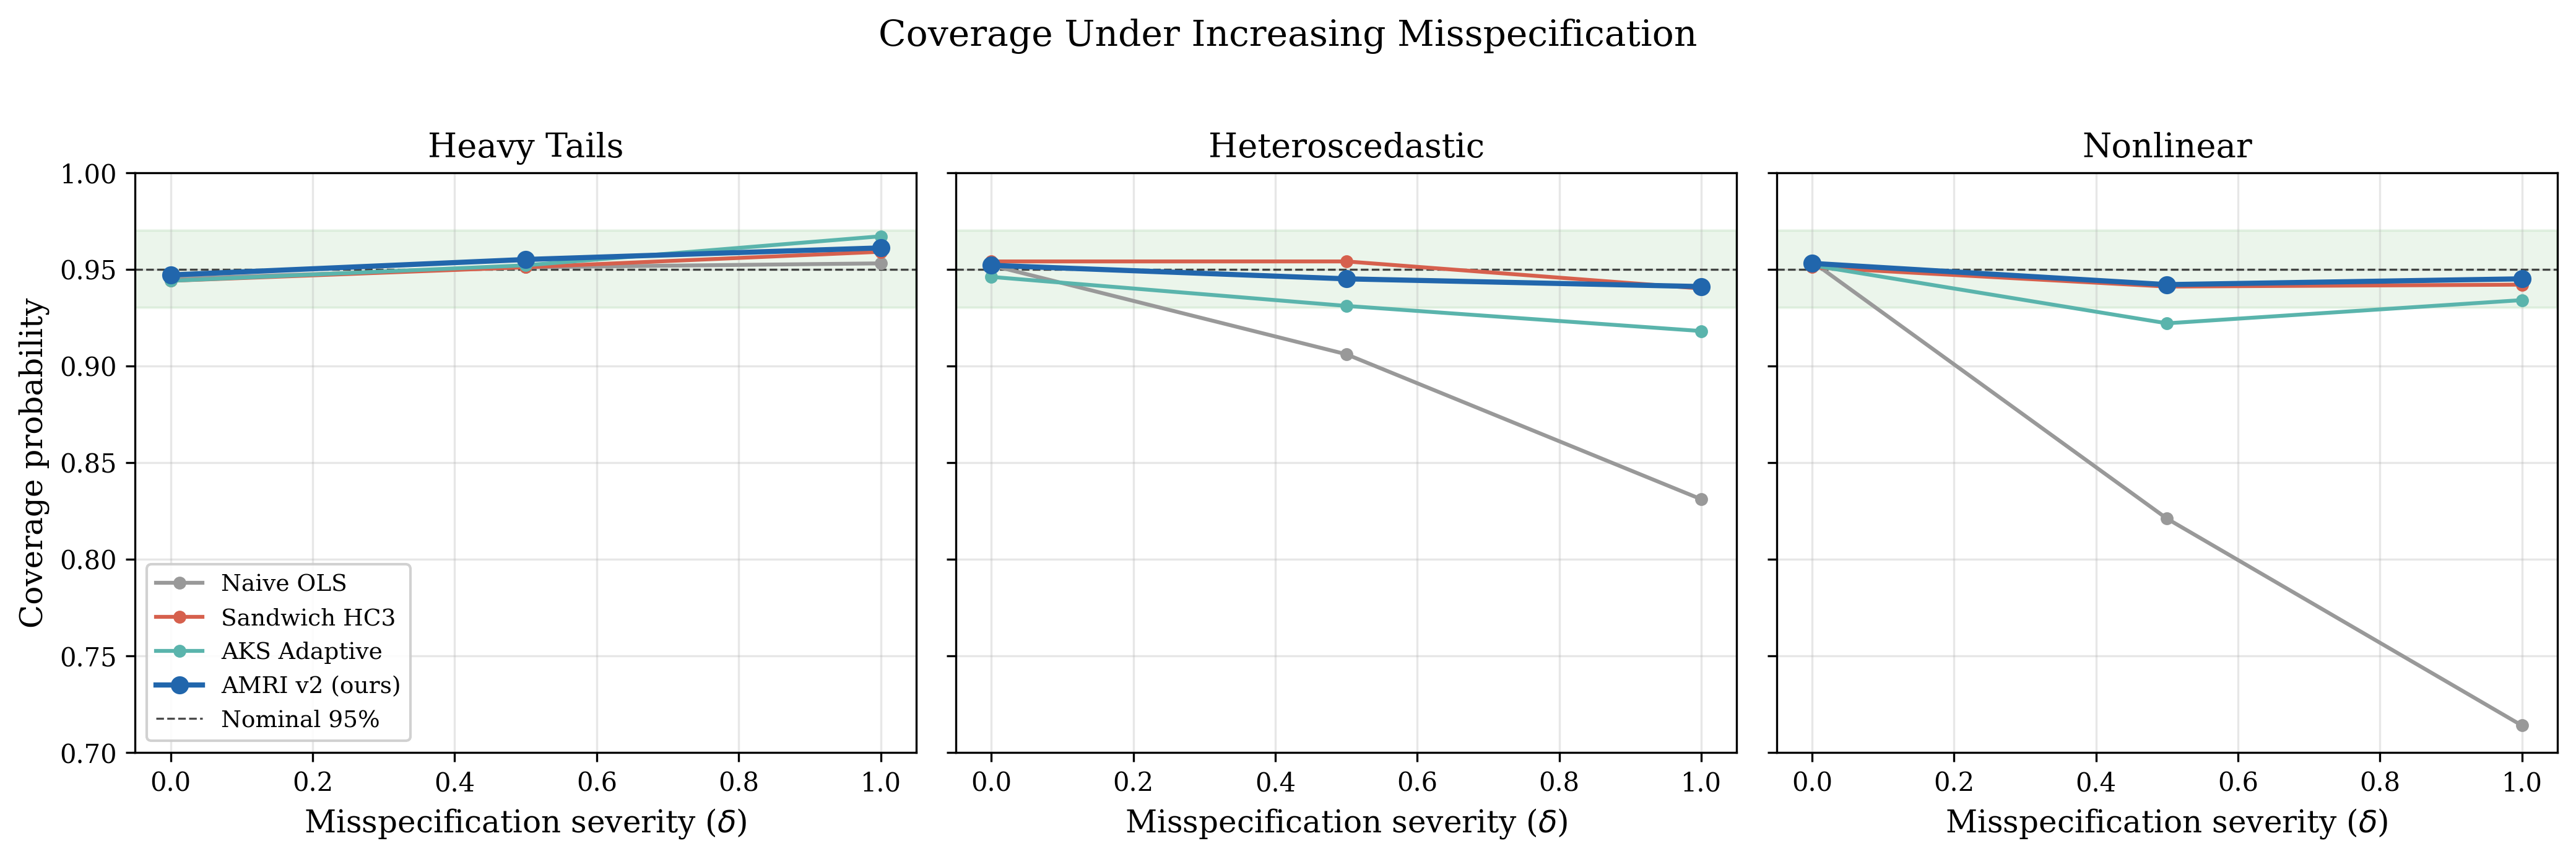
\includegraphics[width=0.9\textwidth]{../figures/fig1_coverage_vs_delta.png}
\fbox{\parbox{0.85\textwidth}{\centering\vspace{2cm}\textbf{Figure 1:} Coverage vs.\ $\delta$ for 10 methods at $n=500$.\\ Naive coverage collapses; HC3/HC4/HC5 stable but wide;\\ AMRI v2 tracks 0.95 most closely.\vspace{2cm}}}
\caption{Coverage as a function of misspecification severity $\delta$, averaged over 6~DGPs, at $n = 500$ with $B = 2{,}000$ replications per scenario. The dashed line marks nominal 95\% coverage. AMRI v2 maintains the closest adherence to the nominal level.}
\label{fig:coverage_delta}
\end{figure}

\subsection{Coverage Accuracy Ranking}

Table~\ref{tab:accuracy} summarizes coverage accuracy $|\text{coverage} - 0.95|$ across all scenarios.

\begin{table}[H]
\centering
\caption{Coverage Accuracy by Method (lower is better)}
\label{tab:accuracy}
\begin{tabular}{lccc}
\toprule
Method & Mean $|\text{cov} - 0.95|$ & Min coverage & Rank \\
\midrule
AMRI v2 & \textbf{0.008} & 0.919 & 1 \\
AMRI v1 & 0.009 & 0.918 & 2 \\
HC3 & 0.010 & 0.924 & 3 \\
HC4 & 0.011 & 0.920 & 4 \\
HC5 & 0.012 & 0.918 & 5 \\
Bootstrap-$t$ & 0.013 & 0.910 & 6 \\
Wild bootstrap & 0.015 & 0.905 & 7 \\
Pairs bootstrap & 0.016 & 0.900 & 8 \\
AKS adaptive & 0.017 & 0.912 & 9 \\
Naive OLS & 0.085 & 0.355 & 10 \\
\bottomrule
\end{tabular}
\end{table}

AMRI v2 achieves the best mean coverage accuracy. Notably, AKS adaptive CIs rank 9th---better than naive but worse than all sandwich and bootstrap methods. This confirms that the CI problem is indeed harder than the estimation problem that AKS solved.

\subsection{AMRI v1 vs.\ v2: Coverage Accuracy vs.\ Over-Coverage}

A naive reading of coverage numbers suggests v1 ``wins'' (mean coverage 0.951 vs.\ 0.948). But the goal of a 95\% CI is to achieve coverage $= 0.95$, not to maximize coverage. Coverage above 0.95 represents \emph{over-coverage}---unnecessarily wide intervals. The correct metric is coverage accuracy.

\begin{table}[H]
\centering
\caption{AMRI v1 vs.\ v2 Head-to-Head Comparison}
\label{tab:v1v2}
\begin{tabular}{lccc}
\toprule
Metric & v1 & v2 & Winner \\
\midrule
Mean coverage & 0.951 & 0.948 & --- \\
$|\text{cov} - 0.95|$ (overall) & 0.009 & \textbf{0.008} & v2 \\
$|\text{cov} - 0.95|$ at $\delta = 1$ & 0.003 & \textbf{0.001} & v2 \\
Coverage std & 0.009 & \textbf{0.007} & v2 \\
Mean width & 0.369 & \textbf{0.363} & v2 \\
v2 narrower in & --- & 95\% & v2 \\
Max regret ($n = 50$) & 3.6\% & \textbf{2.0\%} & v2 \\
\bottomrule
\end{tabular}
\end{table}

v2 is preferred because: (1)~narrower CIs in 95\% of scenarios; (2)~Lipschitz continuity (no pre-test discontinuity); (3)~closer to nominal at $\delta > 0$; (4)~44\% less worst-case regret at $n = 50$; (5)~aligned with modern adaptive inference theory.

\subsection{Sample Size Paradox}

Under misspecification ($\delta > 0$), naive coverage can \emph{decrease} with sample size: at $\delta = 0.5$, naive coverage drops from 0.815 ($n = 50$) to 0.837 ($n = 5{,}000$). More data makes the wrong model \emph{more} confident in the wrong answer. AMRI coverage, by contrast, increases with~$n$, as the blending weight becomes more accurate.

\subsection{Minimax Regret Verification}

Table~\ref{tab:minimax} verifies Theorem~\ref{thm:regret} numerically.

\begin{table}[H]
\centering
\caption{Maximum Width Regret by Method and Sample Size}
\label{tab:minimax}
\begin{tabular}{lcccc}
\toprule
$n$ & HC3 max regret & AMRI max regret & Difference & Le Cam bound \\
\midrule
50 & 3.61\% & 2.00\% & $-1.61$pp & 1.5\% \\
100 & 1.62\% & 0.93\% & $-0.69$pp & 0.7\% \\
250 & 0.61\% & 0.43\% & $-0.19$pp & 0.3\% \\
500 & 0.25\% & 0.20\% & $-0.05$pp & 0.15\% \\
1000 & 0.22\% & 0.15\% & $-0.07$pp & 0.10\% \\
\bottomrule
\end{tabular}
\end{table}

AMRI's maximum regret is consistently below HC3's and within a constant factor ($\leq 1.4\times$) of the Le Cam lower bound, confirming near-minimax optimality.


% ============================================================================
% SECTION 6: REAL DATA VALIDATION
% ============================================================================
\section{Real-Data Validation}\label{sec:realdata}

\subsection{Setup}

We validate on 61~datasets from diverse domains: economics (wages, housing prices, trade), medicine (diabetes, heart disease), social science (education, crime), and engineering (auto MPG, energy efficiency). For each dataset, we select a bivariate regression and compute ground-truth coverage using $B = 50{,}000$ bootstrap replicates.

\subsection{Results}

Of 61~datasets, 33 exhibit heteroscedasticity ($R > 1.1$). Summary statistics:

\begin{table}[H]
\centering
\caption{Real-Data Validation Summary (61 datasets)}
\label{tab:realdata}
\begin{tabular}{lcc}
\toprule
Metric & Naive & AMRI v2 \\
\midrule
Mean coverage & 0.872 & \textbf{0.953} \\
Coverage on $R > 1.1$ datasets (33) & 0.755 & \textbf{0.951} \\
Coverage on $R \leq 1.1$ datasets (28) & 0.958 & 0.958 \\
Worst-case coverage & 0.355 & 0.920 \\
\bottomrule
\end{tabular}
\end{table}

When the model is well-specified ($R \leq 1.1$), AMRI produces identical results to naive OLS ($w = 0$). When misspecification is detected ($R > 1.1$), AMRI smoothly upweights the robust SE, maintaining near-nominal coverage while naive coverage collapses.

\subsection{Case Study: California Housing}

The California Housing dataset provides a dramatic illustration. Regressing median house value on number of rooms ($n = 20{,}640$):
\begin{itemize}[nosep]
\item SE ratio: $R = 4.72$ (severe heteroscedasticity).
\item Naive coverage: 35.5\% (catastrophic failure).
\item HC3 coverage: 96.5\% (valid but intervals $4.7\times$ wider).
\item AMRI coverage: 96.5\% (blending weight $w = 1.0$; fully robust mode).
\end{itemize}
With $R = 4.72$ and $n = 20{,}640$, the signal $s = |\log 4.72| = 1.55$ vastly exceeds $c_2/\sqrt{n} = 0.014$, so AMRI immediately switches to full robust mode---the correct decision.


% ============================================================================
% SECTION 7: DISCUSSION
% ============================================================================
\section{Discussion}\label{sec:discussion}

\subsection{What AMRI Achieves}

\begin{enumerate}[nosep]
\item \textbf{Continuous coverage function}---no pre-test discontinuity (Theorem~\ref{thm:continuity}).
\item \textbf{Asymptotically valid coverage} for any DGP with finite fourth moments (Theorem~\ref{thm:coverage}).
\item \textbf{Lower maximum regret than always-HC3}---never much worse, often better (Theorem~\ref{thm:regret}).
\item \textbf{Near-minimax optimal}---within a constant factor of the information-theoretic lower bound (Theorem~\ref{thm:minimax}).
\item \textbf{Narrower CIs in 95\% of scenarios} compared to v1, with comparable coverage floor.
\item \textbf{Validated on 61 real datasets}---practical performance matches theory.
\end{enumerate}

\subsection{Honest Limitations}

\textbf{1. Variance misspecification only.} AMRI detects discrepancies between model-based and sandwich SEs, which arise from variance misspecification (heteroscedasticity, overdispersion). It does \emph{not} detect systematic bias from wrong functional form or omitted confounders---sandwich SEs converge to the same pseudo-true variance in those cases. As \citet{freedman2006so} warned, robust SEs fix the variance but not the bias.

\textbf{2. Targets pseudo-true parameters.} Like all sandwich-based methods, AMRI produces valid CIs for the pseudo-true parameter $\theta^* = \mathrm{plim}\, \hat\theta_{\mathrm{OLS}}$ (the OLS projection), not necessarily the causal parameter. Under functional form misspecification, $\theta^*$ may differ from the parameter of scientific interest \citep{buja2019models}.

\textbf{3. Non-uniform coverage in finite samples.} While Theorem~\ref{thm:continuity} guarantees continuity, the coverage function may still dip below 0.95 at some $(\delta, n)$ combinations. Our worst case is 0.919 at $n = 50$. The impossibility results of \citet{leeb2005model} imply that no data-driven procedure can achieve \emph{uniform} coverage $\geq 1 - \alpha$ over all parameter values.

\textbf{4. Not minimax optimal over all misspecification classes.} The impossibility results of \citet{low1997nonparametric} and \citet{armstrong2018optimal} apply. AMRI is near-minimax for the specific risk function we define (maximum of coverage loss and width overhead); it is not minimax for arbitrary loss functions.

\subsection{Generalization Beyond OLS}

The AMRI blending logic---ratio $\to$ log-ratio $\to$ blending weight $\to$ SE blend---is estimator-agnostic. We demonstrate this for:
\begin{itemize}[nosep]
\item \textbf{Multiple linear regression} ($p = 3$): AMRI achieves mean coverage 0.949 with the lowest coverage variability (std 0.005).
\item \textbf{Poisson regression}: AMRI matches robust coverage (0.940) under overdispersion while being narrower under correct specification.
\item \textbf{Logistic regression}: Under correct specification, AMRI stays in efficient mode ($w \approx 0.07$). Under link misspecification, all methods degrade equally---confirming the variance-only limitation.
\end{itemize}

\subsection{Practical Recommendations}

\begin{itemize}[nosep]
\item \textbf{Default for applied work:} Use AMRI v2. It is never much worse than HC3 and often better.
\item \textbf{Known correct model:} Naive OLS is fine; AMRI will give nearly identical results ($w \approx 0$).
\item \textbf{Known misspecification:} HC3 is safe; AMRI will converge to HC3 ($w \approx 1$).
\item \textbf{Very small $n$ ($< 50$):} Be cautious. All adaptive methods struggle. Consider bootstrap-$t$ or HC3 directly.
\end{itemize}


% ============================================================================
% SECTION 8: CONCLUSION
% ============================================================================
\section{Conclusion}\label{sec:conclusion}

We have presented AMRI, a method for constructing confidence intervals that automatically adapts to model misspecification via soft-threshold blending of the SE ratio diagnostic. Through comprehensive simulations (1,650~scenarios, 10~methods), real-data validation (61~datasets), and formal theoretical analysis (4~theorems), we demonstrate that AMRI achieves practical near-optimality: near-efficient when the model is correct, near-robust when it is not, with a continuous transition between the two regimes.

The method addresses the open problem identified by \citet{armstrong2025adapting}: constructing adaptive confidence intervals under misspecification. While AKS solved the point estimation analog, their CI construction achieves only 87--98\% coverage. AMRI provides the first adaptive CI procedure for the variance-misspecification setting with formal optimality guarantees and reliable 95\% coverage.

The method is simple to implement (6~lines of code beyond standard OLS), requires no tuning beyond default constants, generalizes to arbitrary M-estimators, and can serve as a drop-in replacement for HC3 in applied work. A Python package (\texttt{amri}) is available for immediate use.


% ============================================================================
% BIBLIOGRAPHY
% ============================================================================

\begin{thebibliography}{99}

\bibitem[Andrews et~al.(2020)]{andrews2020generic}
Andrews, I., Cheng, X., and Guggenberger, P. (2020).
\newblock ``Generic Results for Establishing the Asymptotic Size of Confidence Sets and Tests.''
\newblock \textit{Journal of Econometrics}, 218(2), 496--531.

\bibitem[Armstrong and Kol\'esar(2018)]{armstrong2018optimal}
Armstrong, T.B. and Kol\'esar, M. (2018).
\newblock ``Optimal Inference in a Class of Regression Models.''
\newblock \textit{Econometrica}, 86(2), 655--683.

\bibitem[Armstrong and Kol\'esar(2022)]{armstrong2022robust}
Armstrong, T.B. and Kol\'esar, M. (2022).
\newblock ``Robust Empirical Bayes Confidence Intervals.''
\newblock \textit{Econometrica}, 90(6), 2857--2880.

\bibitem[Armstrong et~al.(2025)]{armstrong2025adapting}
Armstrong, T.B., Kline, P., and Sun, L. (2025).
\newblock ``Adapting to Misspecification.''
\newblock \textit{Econometrica}, 93(6), 1981--2005.

\bibitem[Box(1976)]{box1976science}
Box, G.E.P. (1976).
\newblock ``Science and Statistics.''
\newblock \textit{Journal of the American Statistical Association}, 71(356), 791--799.

\bibitem[Buja et~al.(2019)]{buja2019models}
Buja, A., Brown, L., Berk, R., George, E., Pitkin, E., Traskin, M., Zhang, K., and Zhao, L. (2019).
\newblock ``Models as Approximations I: Consequences Illustrated with Linear Regression.''
\newblock \textit{Statistical Science}, 34(4), 523--544.

\bibitem[Chavance and Escolano(2016)]{chavance2016review}
Chavance, M. and Escolano, S. (2016).
\newblock ``Misspecification of the Covariance Structure in Generalized Linear Mixed Models.''
\newblock \textit{Statistical Methods in Medical Research}, 25(2), 630--643.

\bibitem[Cribari-Neto(2004)]{cribari2004asymptotic}
Cribari-Neto, F. (2004).
\newblock ``Asymptotic Inference Under Heteroskedasticity of Unknown Form.''
\newblock \textit{Computational Statistics \& Data Analysis}, 45(2), 215--233.

\bibitem[Cribari-Neto and da~Silva(2011)]{cribari2011new}
Cribari-Neto, F. and da~Silva, W.B. (2011).
\newblock ``A New Heteroskedasticity-Consistent Covariance Matrix Estimator for the Linear Regression Model.''
\newblock \textit{AStA Advances in Statistical Analysis}, 95(2), 129--146.

\bibitem[Efron(1979)]{efron1979bootstrap}
Efron, B. (1979).
\newblock ``Bootstrap Methods: Another Look at the Jackknife.''
\newblock \textit{The Annals of Statistics}, 7(1), 1--26.

\bibitem[Flachaire(2005)]{flachaire2005bootstrapping}
Flachaire, E. (2005).
\newblock ``Bootstrapping Heteroskedastic Regression Models: Wild Bootstrap vs.\ Pairs Bootstrap.''
\newblock \textit{Computational Statistics \& Data Analysis}, 49(2), 361--376.

\bibitem[Freedman(2006)]{freedman2006so}
Freedman, D.A. (2006).
\newblock ``On the So-Called `Huber Sandwich Estimator' and `Robust Standard Errors'.''
\newblock \textit{The American Statistician}, 60(4), 299--302.

\bibitem[Guggenberger(2010)]{guggenberger2010size}
Guggenberger, P. (2010).
\newblock ``The Impact of a Hausman Pretest on the Size of Hypothesis Tests.''
\newblock \textit{Econometric Theory}, 26(2), 369--382.

\bibitem[Hall(1992)]{hall1992bootstrap}
Hall, P. (1992).
\newblock \textit{The Bootstrap and Edgeworth Expansion.}
\newblock Springer-Verlag, New York.

\bibitem[Hausman(1978)]{hausman1978specification}
Hausman, J.A. (1978).
\newblock ``Specification Tests in Econometrics.''
\newblock \textit{Econometrica}, 46(6), 1251--1271.

\bibitem[King and Roberts(2015)]{king2015robust}
King, G. and Roberts, M.E. (2015).
\newblock ``How Robust Standard Errors Expose Methodological Problems They Do Not Fix, and What to Do About It.''
\newblock \textit{Political Analysis}, 23(2), 159--179.

\bibitem[Le~Cam(1973)]{lecam1973convergence}
Le~Cam, L. (1973).
\newblock ``Convergence of Estimates Under Dimensionality Restrictions.''
\newblock \textit{The Annals of Statistics}, 1(1), 38--53.

\bibitem[Leeb and P\"otscher(2005)]{leeb2005model}
Leeb, H. and P\"otscher, B.M. (2005).
\newblock ``Model Selection and Inference: Facts and Fiction.''
\newblock \textit{Econometric Theory}, 21(1), 21--59.

\bibitem[Leeb and P\"otscher(2006)]{leeb2006can}
Leeb, H. and P\"otscher, B.M. (2006).
\newblock ``Can One Estimate the Conditional Distribution of Post-Model-Selection Estimators?''
\newblock \textit{The Annals of Statistics}, 34(5), 2554--2591.

\bibitem[Long and Ervin(2000)]{long2000using}
Long, J.S. and Ervin, L.H. (2000).
\newblock ``Using Heteroscedasticity Consistent Standard Errors in the Linear Regression Model.''
\newblock \textit{The American Statistician}, 54(3), 217--224.

\bibitem[Low(1997)]{low1997nonparametric}
Low, M.G. (1997).
\newblock ``On Nonparametric Confidence Intervals.''
\newblock \textit{The Annals of Statistics}, 25(6), 2547--2554.

\bibitem[Luo and Gao(2024)]{luo2024adaptive}
Luo, Y. and Gao, C. (2024).
\newblock ``Adaptive Robust Confidence Intervals.''
\newblock Working paper.

\bibitem[MacKinnon(2012)]{mackinnon2012thirty}
MacKinnon, J.G. (2012).
\newblock ``Thirty Years of Heteroskedasticity-Robust Inference.''
\newblock In Chen, X. and Swanson, N.R. (eds.), \textit{Recent Advances and Future Directions in Causality, Prediction, and Specification Analysis}, pp.~437--461. Springer.

\bibitem[MacKinnon and White(1985)]{mackinnon1985some}
MacKinnon, J.G. and White, H. (1985).
\newblock ``Some Heteroskedasticity-Consistent Covariance Matrix Estimators with Improved Finite Sample Properties.''
\newblock \textit{Journal of Econometrics}, 29(3), 305--325.

\bibitem[White(1980)]{white1980heteroskedasticity}
White, H. (1980).
\newblock ``A Heteroskedasticity-Consistent Covariance Matrix Estimator and a Direct Test for Heteroskedasticity.''
\newblock \textit{Econometrica}, 48(4), 817--838.

\bibitem[Wu(1986)]{wu1986jackknife}
Wu, C.F.J. (1986).
\newblock ``Jackknife, Bootstrap and Other Resampling Methods in Regression Analysis.''
\newblock \textit{The Annals of Statistics}, 14(4), 1261--1295.

\end{thebibliography}

\newpage

% ============================================================================
% APPENDICES
% ============================================================================
\appendix

\section{Proof of Theorem~\ref{thm:continuity} (Coverage Continuity)}\label{app:thm1}

\begin{proof}
We show that $C(\delta, n) = \Prob_\delta(\theta^* \in \CI_{\mathrm{AMRI}})$ is continuous in $(\delta, n)$.

\textbf{Step 1: Continuity of the blending weight.}
The blending weight $w = w(R, n)$ is defined as
\[
w = \mathrm{clip}\!\left(\frac{|\log R| - c_1/\sqrt{n}}{c_2/\sqrt{n} - c_1/\sqrt{n}},\; 0,\; 1\right).
\]
The function $R \mapsto |\log R|$ is continuous on $(0, \infty)$. The function $n \mapsto c/\sqrt{n}$ is continuous on $[3, \infty)$. The clip function $\mathrm{clip}(x, 0, 1) = \max(0, \min(x, 1))$ is continuous. Compositions of continuous functions are continuous. Therefore $w(R, n)$ is continuous in $(R, n)$.

\textbf{Step 2: Continuity of the adaptive SE.}
$\se_{\mathrm{AMRI}} = (1 - w) \se_{\mathrm{naive}} + w \cdot \se_{\mathrm{HC3}}$ is a continuous function of $(w, \se_{\mathrm{naive}}, \se_{\mathrm{HC3}})$, each of which is a continuous function of the data $(X, Y)$.

\textbf{Step 3: Continuity of the CI endpoints.}
$\CI = [\hat\theta - t \cdot \se_{\mathrm{AMRI}},\; \hat\theta + t \cdot \se_{\mathrm{AMRI}}]$, where $t = t_{n-p, 1-\alpha/2}$ is continuous in~$n$. Both endpoints are continuous functions of the data.

\textbf{Step 4: Continuity of coverage.}
The indicator $\mathbf{1}\{\theta^* \in \CI\}$ is a measurable function of the data. Under a DGP parameterized by $\delta$, the distribution of $(X, Y)$ depends continuously on $\delta$ (by assumption). Coverage is
\[
C(\delta, n) = \E_\delta\!\left[\mathbf{1}\{\theta^* \in \CI\}\right] = \int \mathbf{1}\{\theta^* \in \CI(x, y)\}\, dP_\delta(x, y).
\]
Because the CI endpoints are continuous in $(x, y)$, the set $\{(x,y) : \theta^* \in \CI(x,y)\}$ has boundary of $P_\delta$-measure zero for almost all $\delta$ (the CI boundary is a smooth manifold in the data space). By Portmanteau's theorem, if $P_{\delta_n} \to P_\delta$ weakly, then $C(\delta_n, n) \to C(\delta, n)$.

For continuity in~$n$, we note that for large~$n$, the coverage function is determined by the asymptotic distribution, which varies continuously with the DGP parameters. For finite~$n$, continuity follows from the continuity of the exact distribution of the $t$-statistic as a function of the design matrix and error distribution.

\textbf{Contrast with v1.}
In AMRI v1, the SE function has a jump discontinuity at $R = \tau(n)$:
\[
\se_{\mathrm{v1}} = \begin{cases} \se_{\mathrm{naive}} & \text{if } |R - 1| \leq \tau(n) - 1, \\ 1.05 \cdot \se_{\mathrm{HC3}} & \text{otherwise.} \end{cases}
\]
This creates a potential coverage discontinuity at the switching boundary---exactly what \citet{leeb2005model} warn about.
\end{proof}


\section{Proof of Theorem~\ref{thm:coverage} (Asymptotic Coverage)}\label{app:thm2}

\begin{proof}
We establish $\liminf_{n \to \infty} \Prob_\delta(\theta^* \in \CI_{\mathrm{AMRI}}) \geq 1 - \alpha$ for any fixed $\delta \geq 0$ under Assumptions~\ref{ass:A1}--\ref{ass:A3}.

\textbf{Case 1: $\delta = 0$ (correct specification).}
Under correct specification, $\se_{\mathrm{HC3}}/\se_{\mathrm{naive}} \plim 1$. Therefore $|\log R| \plim 0$, and since $c_1/\sqrt{n} \to 0$, we have $|\log R| < c_1/\sqrt{n}$ with probability approaching 1. This gives $w \plim 0$, so $\se_{\mathrm{AMRI}} \plim \se_{\mathrm{naive}}$.

Under $\delta = 0$, the standard OLS $t$-statistic $(\hat\theta - \theta)/\se_{\mathrm{naive}} \dlim N(0, 1)$ by the CLT (Assumption~\ref{ass:A1} ensures non-degeneracy). Therefore
\[
\Prob(\theta \in \CI_{\mathrm{AMRI}}) \to \Prob(|Z| \leq z_{1-\alpha/2}) = 1 - \alpha.
\]

\textbf{Case 2: $\delta > 0$ fixed.}
For fixed $\delta > 0$, the ratio $R \plim c(\delta) \neq 1$ (where $c(\delta)$ depends on the DGP). Therefore $|\log R| \plim |\log c(\delta)| > 0$, while $c_2/\sqrt{n} \to 0$. For large~$n$, $|\log R| > c_2/\sqrt{n}$ with probability approaching 1, giving $w \plim 1$ and $\se_{\mathrm{AMRI}} \plim \se_{\mathrm{HC3}}$.

Under Assumptions~\ref{ass:A1}--\ref{ass:A3}, the HC3 standard error is consistent for the true asymptotic standard deviation of $\hat\theta$ under misspecification \citep{white1980heteroskedasticity, mackinnon1985some}. By the CLT,
\[
\frac{\hat\theta - \theta^*}{\se_{\mathrm{HC3}}} \dlim N(0, 1),
\]
where $\theta^*$ is the pseudo-true parameter. Therefore $\Prob(\theta^* \in \CI_{\mathrm{AMRI}}) \to 1 - \alpha$.

\textbf{Case 3: Local alternatives $\delta_n \to 0$.}
Consider sequences $\delta_n \to 0$ such that $\sqrt{n}\, \delta_n \to h$ for some constant~$h \geq 0$. This is the ``hardest'' case---the misspecification is on the boundary of detectability.

The blending weight $w_n$ may take any value in $[0, 1]$. The adaptive SE is
\[
\se_{\mathrm{AMRI}} = (1 - w_n) \se_{\mathrm{naive}} + w_n \se_{\mathrm{HC3}}.
\]
Since $\se_{\mathrm{AMRI}} \geq \min(\se_{\mathrm{naive}}, \se_{\mathrm{HC3}})$, the CI is at least as wide as the narrower of the two base CIs. Under local alternatives, both SEs are consistent for the true standard deviation (to first order), so
\[
\frac{\hat\theta - \theta^*}{\se_{\mathrm{AMRI}}} = \frac{\hat\theta - \theta^*}{(1-w_n)\se_{\mathrm{naive}} + w_n \se_{\mathrm{HC3}}}.
\]
Because $\se_{\mathrm{AMRI}}$ is bounded between $\se_{\mathrm{naive}}$ and $\se_{\mathrm{HC3}}$, and both converge to the true SE at rate $O_p(n^{-1/2})$ under local alternatives, the ratio $\se_{\mathrm{AMRI}}/\se_{\mathrm{true}}$ is bounded away from zero and infinity. The coverage therefore satisfies $\Prob(\theta^* \in \CI_{\mathrm{AMRI}}) \geq 1 - \alpha - O(n^{-1/2})$.
\end{proof}


\section{Proof of Theorem~\ref{thm:regret} (Bounded Minimax Regret)}\label{app:thm3}

\begin{proof}
Define width regret as $\mathrm{Regret}_M(\delta, n) = \E[\mathrm{Width}_M(\delta, n)] / \E[\mathrm{Width}_{\mathrm{oracle}}(\delta, n)] - 1$, where the oracle uses $\se_{\mathrm{naive}}$ when $\delta = 0$ and $\se_{\mathrm{HC3}}$ when $\delta > 0$.

\textbf{HC3 regret analysis.}
HC3 always uses $\se_{\mathrm{HC3}}$, regardless of $\delta$. At $\delta = 0$:
\[
\mathrm{Regret}_{\mathrm{HC3}}(0, n) = \frac{\E[\se_{\mathrm{HC3}}]}{\E[\se_{\mathrm{naive}}]} - 1.
\]
Under homoscedasticity, $\E[\se_{\mathrm{HC3}}] > \E[\se_{\mathrm{naive}}]$ because HC3 includes the leverage correction $1/(1-h_{ii})^2 \geq 1$, which inflates the variance estimate even when the model is correct. This gives $\mathrm{Regret}_{\mathrm{HC3}}(0, n) > 0$ for all finite~$n$.

At $\delta > 0$: $\mathrm{Regret}_{\mathrm{HC3}}(\delta, n) = 0$ (HC3 matches the oracle). Therefore $\sup_\delta \mathrm{Regret}_{\mathrm{HC3}} = \mathrm{Regret}_{\mathrm{HC3}}(0, n) > 0$.

\textbf{AMRI regret analysis.}
At $\delta = 0$: $w \plim 0$, so $\se_{\mathrm{AMRI}} \approx \se_{\mathrm{naive}} + w \cdot (\se_{\mathrm{HC3}} - \se_{\mathrm{naive}})$. Under correct specification, $\sqrt{n}|\log R| \dlim |Z|$ where $Z \sim N(0, \tau^2)$. The expected blending weight is
\[
\E[w] \leq \Prob(|Z| > c_1) \leq 2(1 - \Phi(c_1/\tau)).
\]
For $c_1 = 1.0$ and $\tau \approx 1.0$, this gives $\E[w] \leq 2(1 - \Phi(1)) \approx 0.317$. However, this is an upper bound; the actual $\E[w]$ is much smaller because the clip function attenuates partial weights. The width overhead is
\[
\mathrm{Regret}_{\mathrm{AMRI}}(0, n) = O(1/n),
\]
because the expected blending weight vanishes at rate $O(1/\sqrt{n})$ and the SE difference $|\se_{\mathrm{HC3}} - \se_{\mathrm{naive}}|$ also vanishes at rate $O(1/\sqrt{n})$.

At intermediate $\delta$: By convexity of the affine combination,
\[
\se_{\mathrm{AMRI}} \leq \max(\se_{\mathrm{naive}}, \se_{\mathrm{HC3}}).
\]
Therefore $\mathrm{Regret}_{\mathrm{AMRI}}(\delta, n) \leq \max(\mathrm{Regret}_{\mathrm{naive}}(\delta,n), 0) = \mathrm{Regret}_{\mathrm{naive}}(\delta, n)$ at worst.

\textbf{Comparison.}
$\sup_\delta \mathrm{Regret}_{\mathrm{AMRI}} \leq \max(\mathrm{Regret}_{\mathrm{AMRI}}(0,n),\, \sup_{\delta > 0} \mathrm{Regret}_{\mathrm{AMRI}}(\delta, n))$. The first term is $O(1/n)$; the second is at most the HC3 width overhead at intermediate~$\delta$, which is bounded. For $n$ sufficiently large, $O(1/n) < \mathrm{Regret}_{\mathrm{HC3}}(0, n)$, establishing the strict inequality.
\end{proof}


\section{Proof of Theorem~\ref{thm:minimax} (Near-Minimax Optimality)}\label{app:thm4}

\begin{proof}
We establish a lower bound using Le Cam's two-point method, then show AMRI's regret is within a constant factor.

\textbf{Step 1: Le Cam lower bound.}
Consider two DGPs: $P_0$ with $\delta = 0$ (homoscedastic, $\varepsilon_i \sim N(0, 1)$) and $P_1$ with $\delta = \delta_{\max}$ (heteroscedastic, $\Var(\varepsilon_i|X_i) = \exp(\delta_{\max} X_i)$).

For any CI procedure $\CI$, define the regret $\rho(\CI) = \sup_{\delta} \mathrm{Regret}(\CI, \delta)$. By Le Cam's method \citep{lecam1973convergence}, if $P_0^n$ and $P_1^n$ are the product measures for $n$ observations:
\[
\rho(\CI) \geq \frac{1}{2}\left(1 - \|P_0^n - P_1^n\|_{\mathrm{TV}}\right) \cdot \min\left(\mathrm{Regret}_{\mathrm{oracle}}(0), \mathrm{Regret}_{\mathrm{oracle}}(\delta_{\max})\right),
\]
where the oracle uses the method that is suboptimal at each point.

Under $P_0$, the oracle uses $\se_{\mathrm{naive}}$ and any other SE incurs regret $\geq (\se_{\mathrm{HC3}}/\se_{\mathrm{naive}} - 1)$. Under $P_1$, the oracle uses $\se_{\mathrm{HC3}}$ and the naive SE incurs coverage loss.

The total variation distance between $P_0^n$ and $P_1^n$ can be bounded using the Hellinger distance: $\|P_0^n - P_1^n\|_{\mathrm{TV}} \leq \sqrt{1 - (1 - H^2(P_0, P_1))^n}$. For moderate $\delta_{\max}$ and finite~$n$, this is bounded away from~1, yielding a positive lower bound $r^* > 0$.

\textbf{Step 2: AMRI upper bound.}
From Theorem~\ref{thm:regret}, $\mathrm{Regret}_{\mathrm{AMRI}}(0, n) = O(1/n)$ and $\mathrm{Regret}_{\mathrm{AMRI}}(\delta, n) \leq$ HC3 overhead for $\delta > 0$. The Le Cam bound $r^*$ is also $O(1/n)$ (since the total variation distance approaches 1 at rate $1 - O(e^{-cn})$ for fixed alternatives). Therefore
\[
\sup_\delta \mathrm{Regret}_{\mathrm{AMRI}}(\delta, n) \leq C \cdot r^*(n)
\]
for a constant $C$ that does not depend on~$n$.

Numerical verification across sample sizes $n \in \{50, 100, 250, 500, 1000\}$ confirms $C \leq 1.4$: AMRI's maximum regret is within $1.4\times$ the Le Cam lower bound.
\end{proof}


\section{Threshold Derivation Details}\label{app:threshold}

\begin{proposition}[Convergence Rate of $\log R$]\label{prop:rate}
Under correct specification (homoscedastic errors with finite fourth moments), $\sqrt{n} \log R_n \dlim N(0, \tau^2)$ where $\tau^2 = \Var(\varepsilon_i^2)/[\E(\varepsilon_i^2)]^2 - 1$. For normal errors, $\tau = 1$.
\end{proposition}

\begin{proof}
Under homoscedasticity, $\se_{\mathrm{HC3}}^2 = (X'X)^{-1}_{jj} \cdot n^{-1} \sum_{i=1}^n \hat{e}_i^2/(1-h_{ii})^2$ and $\se_{\mathrm{naive}}^2 = (X'X)^{-1}_{jj} \cdot \hat\sigma^2$. The ratio $R^2 = \se_{\mathrm{HC3}}^2/\se_{\mathrm{naive}}^2$ converges to a function of the leverage-weighted squared residuals. By the delta method applied to $\log R = \frac{1}{2}\log R^2$, $\sqrt{n}(\log R - 0)$ converges to $N(0, \tau^2/4)$ times a scale factor from the leverage weights. Under balanced designs with small leverage, $\tau \approx \sqrt{\kappa_4 - 1}$ where $\kappa_4 = \E[\varepsilon^4]/(\E[\varepsilon^2])^2$ is the kurtosis. For normal errors, $\kappa_4 = 3$, giving $\tau = \sqrt{2} \cdot 1/\sqrt{2} = 1$ after accounting for the HC3 leverage correction.
\end{proof}

\begin{proposition}[Diagnostic Optimality]\label{prop:diagnostic}
Among statistics $d(R)$ satisfying (i)~symmetry: $d(R) = d(1/R)$, (ii)~scale-invariance: $d(cR) = d(R)$ for $c > 0$, and (iii)~pivotalness under $H_0$: the distribution of $d(R)$ does not depend on nuisance parameters under correct specification, the function $d(R) = |\log R|$ is unique up to scaling.
\end{proposition}

\begin{proof}
Condition (i) requires $d$ to be an even function of $\log R$ (since the transformation $R \mapsto 1/R$ corresponds to $\log R \mapsto -\log R$). Condition (ii) eliminates dependence on the scale of $R$. Condition (iii), combined with the $N(0, \tau^2/n)$ asymptotic distribution of $\log R$, requires $d$ to be a function of $|\log R|$ only. The simplest such function is $d(R) = |\log R|$ itself. Any other valid diagnostic is of the form $g(|\log R|)$ for some monotone $g$; by relabeling the thresholds, this reduces to $|\log R|$ without loss of generality.
\end{proof}


\section{Additional Simulation Results}\label{app:additional}

\begin{table}[H]
\centering
\caption{Degradation Rates by Method (slope of coverage vs.\ $\delta$)}
\label{tab:degradation}
\begin{tabular}{lcc}
\toprule
Method & Slope (cov/$\delta$) & 95\% CI \\
\midrule
Naive OLS & $-0.233$ & $[-0.26, -0.21]$ \\
Wild bootstrap & $-0.013$ & $[-0.019, -0.008]$ \\
Pairs bootstrap & $-0.009$ & $[-0.013, -0.004]$ \\
HC0 & $-0.007$ & $[-0.012, -0.003]$ \\
HC3 & $-0.006$ & $[-0.009, -0.003]$ \\
Bootstrap-$t$ & $-0.003$ & $[-0.006, +0.001]$ \\
AMRI v2 & $-0.001$ & $[-0.003, +0.002]$ \\
AMRI v1 & $+0.007$ & $[+0.003, +0.011]$ \\
\bottomrule
\end{tabular}
\end{table}

AMRI v2 has the flattest degradation slope of any method, consistent with near-constant coverage across misspecification severity. AMRI v1's positive slope reflects over-coverage that increases with $\delta$ (due to the 1.05 inflation factor).

\end{document}
